\autsection{Salinity \& pH Sensor}{Kristian Sloth Lauszus and Lukas Christensen}
As previously noted, the pH and salinity of an environment is believed to play a large part in the formation of life. Therefore, sensors able to measure these quantities are an integral part of the instrument contingency of this mission. 

\subsection{Technologies}
There exists multiple ways to perform electronic measurements of pH and salinity, however, most of them follow the same basic principle and are more or less variations of the Ion Sensitive Electrode (ICE).\\

\todo[inline]{describe ICE}

\noindent
Other more exotic devices for pH and salinity measurement exist, such as for example voltammetry\cite{website:senova} and holography\cite{article:marshall2003a} based ones. While these devices show great promise and overcome some of the issues associated with ICEs, they are still in their infancy compared to the extremely well characterized ICE systems. Because of this, as well as the fact that they have successfully been used in space before\cite{article:jgre2487}, the design for this mission will be based on ion sensitive electrodes. 

\subsection{Implementation}
* pH
	* Solid state (ISFET)
		* No calibration
		* Measures current flow at different voltages, H+ ions
	* Temperature compensated [5:50] degrees C
		* Response time ~60 s
	* 200 uL, ~20 mW, below 10 mA
	* $\pm$ 0.01 pH
* Salinity can use same instruments using membranes
	* Current flow
* Temperature probe
	* K-type thermal couple

\begin{figure}[htb]
	\centering
	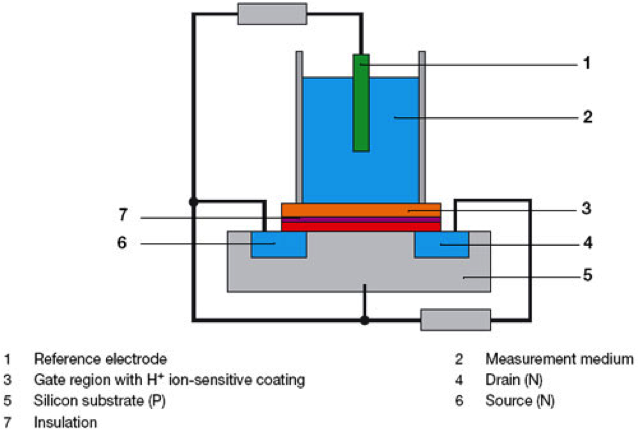
\includegraphics[width=\textwidth]{figures/ISFET.png}
	\caption{TODO: Caption}
	\label{fig:ISFET}
\end{figure}

\subsection{Discussion}
